\begin{frame}
  \frametitle{What is Git?}
  \begin{itemize}
  \item A version control system, like CVS, SVN, Perforce or ClearCase
  \item Originally developed for the Linux kernel development, now
    used by a large number of projects, including U-Boot, GNOME,
    Buildroot, uClibc and many more
  \item Contrary to CVS or SVN, Git is a distributed version control
    system
    \begin{itemize}
    \item No central repository
    \item Everybody has a local repository
    \item Local branches are possible, and very important
    \item Easy exchange of code between developers
    \item Well-suited to the collaborative development model used in
      open-source projects
    \end{itemize}
  \end{itemize}
\end{frame}

\begin{frame}
  \frametitle{Install and Setup}
  \begin{itemize}
  \item Git is available as a package in your distribution
    \begin{itemize}
    \item \code{sudo apt install git}
    \end{itemize}
  \item Everything is available through the git command
    \begin{itemize}
    \item \code{git} has many commands, called using
      \code{git <command>}, where \code{<command>} can be
      \code{clone}, \code{checkout}, \code{branch}, etc.
    \item Help can be found for a given command using
      \code{git help <command>}
    \end{itemize}
  \item Set up your name and e-mail address
    \begin{itemize}
    \item They will be referenced in each of your commits
    \item \code{git config --global user.name 'My Name'}
    \item \code{git config --global user.email me@mydomain.net}
    \end{itemize}
  \end{itemize}
\end{frame}

\begin{frame}
  \frametitle{Clone a Repository}
  \begin{itemize}
  \item To start working on a project, you use Git's clone operation.
  \item With CVS or SVN, you would have used the checkout operation,
    to get a working copy of the project (latest version)
  \item With Git, you get a full copy of the repository, including the
    history, which allows to perform most of the operations offline.
  \item Cloning Linus Torvalds' Linux kernel repository
    \code{git clone git://git.kernel.org/pub/scm/linux/kernel/git/torvalds/linux.git}
  \item \code{git://} is a special Git protocol. Most repositories can
    also be accessed using \code{http://}, but this is slower.
  \item After cloning, in \code{linux/}, you have the repository and a
    working copy of the master branch.
  \end{itemize}
\end{frame}

\begin{frame}[fragile]
  \frametitle{Explore the History}
  \begin{itemize}
  \item \code{git log} will list all the commits. The latest commit is
    the first.
{\scriptsize
\begin{verbatim}
commit 4371ee353c3fc41aad9458b8e8e627eb508bc9a3
Author: Florian Fainelli <florian@openwrt.org>
Date: Mon Jun 1 02:43:17 2009 -0700

MAINTAINERS: take maintainership of the cpmac Ethernet driver

This patch adds me as the maintainer of the CPMAC (AR7)
Ethernet driver.

Signed-off-by: Florian Fainelli <florian@openwrt.org>
Signed-off-by: David S. Miller <davem@davemloft.net>
\end{verbatim}
}
  \item \code{git log -p} will list the commits with the corresponding
    diff
  \item The history in Git is not linear like in CVS or SVN, but it is
    a graph of commits
    \begin{itemize}
    \item Makes it a little bit more complicated to understand at the
      beginning
    \item But this is what allows the powerful features of Git
      (distributed, branching, merging)
    \end{itemize}
  \end{itemize}
\end{frame}

\begin{frame}
  \frametitle{Visualize the History: gitk}
  \begin{itemize}
  \item \code{gitk} is a graphical tool that represents the history of
    the current Git repository
  \item Can be installed from the \code{gitk} package
  \end{itemize}
  \begin{center}
    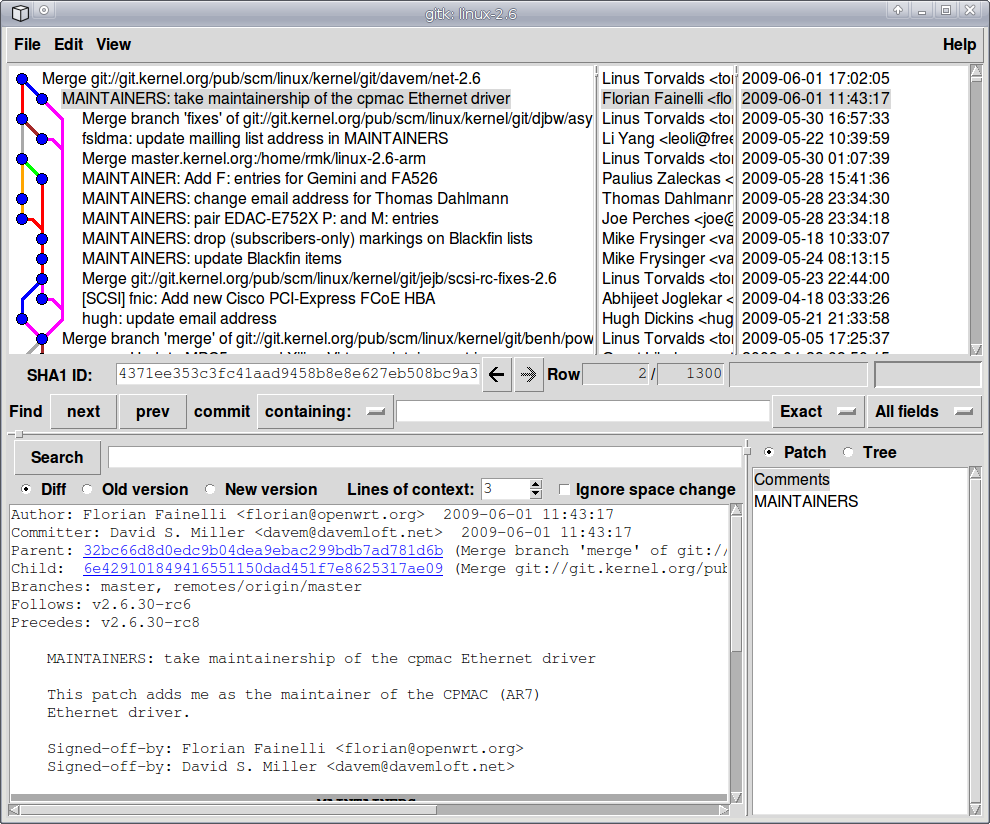
\includegraphics[height=0.65\textheight]{slides/kernel-git-content/gitk.png}
  \end{center}
\end{frame}

\begin{frame}
  \frametitle{Visualize the History: cgit}
  \begin{itemize}
  \item Another great tool is cgit, a web interface to Git. For the
    kernel sources, it is used on \url{https://git.kernel.org/}
  \end{itemize}
  \begin{center}
    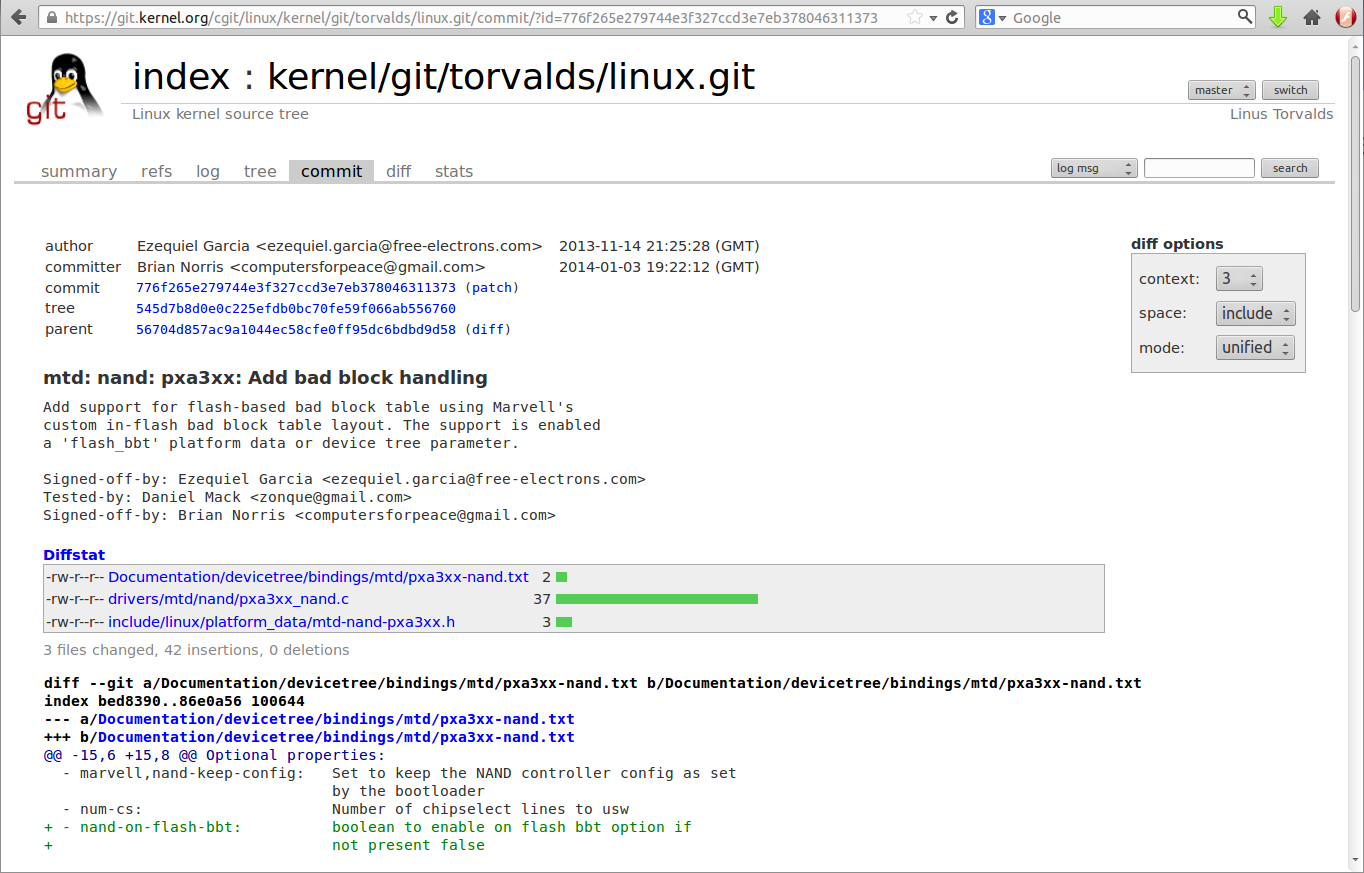
\includegraphics[height=0.65\textheight]{slides/kernel-git-content/git-kernel-org.png}
  \end{center}
\end{frame}

\begin{frame}
  \frametitle{Update your Repository}
  \begin{itemize}
  \item The repository that has been cloned at the beginning will
    change over time
  \item Updating your local repository to reflect the changes of the
    remote repository will be necessary from time to time
  \item \code{git pull}
  \item Internally, does two things
    \begin{itemize}
    \item Fetch the new changes from the remote repository
      (\code{git fetch})
    \item Merge them in the current branch (\code{git merge})
    \end{itemize}
  \end{itemize}
\end{frame}

\begin{frame}
  \frametitle{Tags}
  \begin{itemize}
  \item The list of existing tags can be found using
    \begin{itemize}
    \item \code{git tag -l}
    \end{itemize}
  \item To check out a working copy of the repository at a given tag
    \begin{itemize}
    \item \code{git checkout <tagname>}
    \end{itemize}
  \item To get the list of changes between a given tag and the latest
    available version
    \begin{itemize}
    \item \code{git log v4.19..master}
    \end{itemize}
  \item List of changes with diff on a given file between two tags
    \begin{itemize}
    \item \code{git log -p v4.18..v4.19 MAINTAINERS}
    \end{itemize}
  \item With gitk
    \begin{itemize}
    \item \code{gitk v4.19..master}
    \end{itemize}
  \end{itemize}
\end{frame}

\begin{frame}
  \frametitle{Branches}
  \begin{itemize}
  \item To start working on something, the best is to make a branch
    \begin{itemize}
    \item It is local-only, nobody except you sees the branch
    \item It is fast
    \item It allows to split your work on different topics, try
      something and throw it away
    \item It is cheap, so even if you think you're doing something
      small and quick, do a branch
    \end{itemize}
  \item Unlike other version control systems, Git encourages the use
    of branches. Don't hesitate to use them.
  \end{itemize}
\end{frame}

\begin{frame}
  \frametitle{Branches}
  \begin{itemize}
  \item Create a branch
    \begin{itemize}
    \item \code{git branch <branchname>}
    \end{itemize}
  \item Move to this branch
    \begin{itemize}
    \item \code{git checkout <branchname>}
    \end{itemize}
  \item Both at once (create and switch to branch)
    \begin{itemize}
    \item \code{git checkout -b <branchname>}
    \end{itemize}
  \item List of local branches
    \begin{itemize}
    \item \code{git branch}
    \end{itemize}
  \item List of all branches, including remote branches
    \begin{itemize}
    \item \code{git branch -a}
    \end{itemize}
  \end{itemize}
\end{frame}

\begin{frame}
  \frametitle{Making Changes}
  \begin{itemize}
  \item Edit a file with your favorite text editor
  \item Get the status of your working copy
    \begin{itemize}
    \item \code{git status}
    \end{itemize}
  \item Git has a feature called the index, which allows you to stage
    your commits before committing them. It allows to commit only part
    of your modifications, by file or even by chunk.
  \item On each modified file
    \begin{itemize}
    \item \code{git add <filename>}
    \end{itemize}
  \item Then commit. No need to be on-line or connected to commit
    \begin{itemize}
    \item Linux requires the -s option to sign your changes
    \item \code{git commit -s}
    \end{itemize}
  \item If all modified files should be part of the commit
    \begin{itemize}
    \item \code{git commit -as}
    \end{itemize}
  \end{itemize}
\end{frame}

\begin{frame}
  \frametitle{Sharing Changes: E-mail}
  \begin{itemize}
  \item The simplest way of sharing a few changes is to send patches
    by e-mail
  \item The first step is to generate the patches
    \begin{itemize}
    \item \code{git format-patch master..<yourbranch>}
    \item Will generate one patch for each of the commits done on
      \code{<yourbranch>}
    \item The patch files will be \code{0001-....}, \code{0002-....},
      etc.
    \end{itemize}
  \item The second step is to send these patches by e-mail
    \begin{itemize}
    \item \code{git send-email --compose --to email@domain.com 00*.patch}
    \end{itemize}
    \begin{itemize}
    \item Required Ubuntu package: \code{git-email}
    \item In a later slide, we will see how to use git config to set
      the SMTP server, port, user and password.
    \end{itemize}
  \end{itemize}
\end{frame}

\begin{frame}
  \frametitle{Sharing Changes: Your Own Repository}
  \begin{itemize}
  \item If you do a lot of changes and want to ease collaboration with
    others, the best is to have your own public repository
  \item Use a git hosting service on the Internet:
    \begin{itemize}
    \item GitLab (\url{https://gitlab.com/})
      \begin{itemize}
      \item Open Source server. Proprietary and commercial extensions
       available.
      \end{itemize}
    \item GitHub (\url{https://github.com/})
      \begin{itemize}
      \item For public repositories. Need to pay for private
        repositories.
      \end{itemize}
    \end{itemize}
  \item Publish on your own web server
    \begin{itemize}
    \item Easy to implement.
    \item Just needs git software on the server and ssh access.
    \item Drawback: only supports http cloning (less efficient)
    \end{itemize}
  \item Set up your own git server
    \begin{itemize}
    \item Most flexible solution.
    \item Today's best solutions are \code{gitolite}
      (\url{https://github.com/sitaramc/gitolite}) for the server and
      \code{cgit} for the web interface
      (\url{https://git.zx2c4.com/cgit/about/}).
    \end{itemize}
  \end{itemize}
\end{frame}

\begin{frame}
  \frametitle{Sharing changes: HTTP Hosting}
  \begin{itemize}
  \item Create a bare version of your repository
    \begin{itemize}
    \item \code{cd /tmp}
    \item \code{git clone --bare ~/project project.git}
    \item \code{touch project.git/git-daemon-export-ok}
    \end{itemize}
  \item Transfer the contents of \code{project.git} to a
    publicly-visible place (reachable read-only by HTTP for everybody,
    and read-write by you through SSH)
  \item Tell people to clone
    \code{https://yourhost.com/path/to/project.git}
  \item Push your changes using
    \begin{itemize}
    \item
      \code{git push ssh://yourhost.com/path/toproject.git srcbranch:destbranch}
    \end{itemize}
  \end{itemize}
\end{frame}

\begin{frame}
  \frametitle{Tracking Remote Trees}
  \begin{itemize}
  \item In addition to the official Linus Torvalds tree, you might
    want to use other development or experimental trees
    \begin{itemize}
    \item The OMAP tree at
      \code{git://git.kernel.org/pub/scm/linux/kernel/git/tmlind/linux-omap.git}
    \item The stable realtime tree at
      \code{git://git.kernel.org/pub/scm/linux/kernel/git/rt/linux-stable-rt.git}
    \end{itemize}
  \item The \code{git remote} command allows to manage remote trees
    \begin{itemize}
    \item
      \code{git remote add rt git://git.kernel.org/pub/scm/ linux/kernel/git/rt/linux-stable-rt.git}
    \end{itemize}
  \item Get the contents of the tree
    \begin{itemize}
    \item \code{git fetch rt}
    \end{itemize}
  \item Switch to one of the branches
    \begin{itemize}
    \item \code{git checkout rt/master}
    \end{itemize}
  \end{itemize}
\end{frame}


\begin{frame}
  \frametitle{git-gui}
  \url{https://www.git-scm.com/docs/git-gui}
  \begin{itemize}
  \item A graphical interface to create and manipulate commits,
    replacing multiple git command-line commands.
  \item Not meant for history browsing (opens \code{gitk}
    when needed).
  \begin{center}
    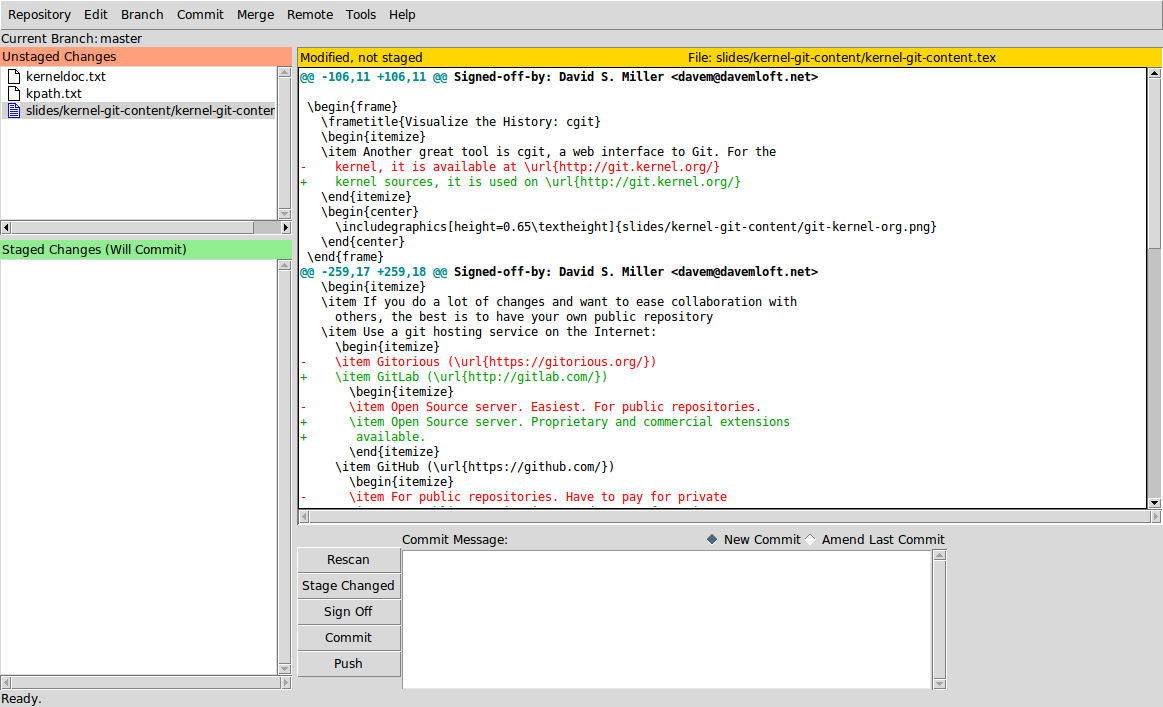
\includegraphics[height=0.45\textheight]{slides/kernel-git-content/git-gui.png}
  \end{center}
  \item Example usage on Ubuntu/Debian:\\
    \code{sudo apt install git-gui}\\
    \code{git gui blame Makefile}
  \end{itemize}
\end{frame}


\begin{frame}
  \frametitle{About Git}
  We have just seen the very basic features of Git.

  Many more interesting features are available (rebasing,
  bisection, merging and more). For more details:
  \begin{columns}
  \column{0.6\textwidth}
    \begin{itemize}
    \item Git Manual
      \newline \url{https://schacon.github.com/git/user-manual.html}
    \item Git Book (freely available on-line, or in print form)
      \newline \url{https://git-scm.com/book}
    \item Git official website
      \newline \url{https://git-scm.com/}
    \item Video: James Bottomley's tutorial on using Git
      \newline \url{https://bit.ly/2fZJxLZ}
    \end{itemize}
  \column{0.4\textwidth}
    
\includegraphics[height=0.45\textheight]{slides/kernel-git-content/progit2.png}
  \end{columns}
\end{frame}
